\chapter{Lab 2: Kalman filter}

\section{Main steps}

\begin{enumerate}
    \item Obtain the matrices  $A_c$, $B_c$,$C_c$ and $D_c$ of the state-space model representing the dynamics of the RLC circuit above, in function of the parameters $R_0$, $L_0$
    and $C_0$. (You can start by applying Kirchoff’s circuit laws in the Laplace domain). Write down the steps performed in the report.
    \item Show the continuous- and discrete-time step responses, and motivate your choice for the sample time. Write down the discretized matrices $A_d$, $B_d$ and $C_d$ in
    the report. Is the system stable? And is it observable?
    \item Simulate the system, using the sampling time $T_s$ selected above and selecting
    the simulation time such that your measurement will have (around) 200 points.
    Choose the input $u(t)$ as white Gaussian noise with standard deviation 1 V. Set (in
    the time-delay block) the initial condition $x_0 =
     \begin{bmatrix}
    0\\
    0
    \end{bmatrix}$.
     Add the names of the blocks inthe Simulink and add a screenshot of it in your report. Extract the true state of the system from the Simulink model.
     \item Compute the state estimates using method a (prediction only) and method b (Kalman filter) - 5 variations.
     \item Comments the results in your report, making sure to provide an answer
    to the following questions. Which method performs better? Which method is more
    robust? Is there a difference in performance between the estimate of the first state
    (voltage capacitor) and of the second state (current) for method a? And for method
    b? Why? What are the effects of the covariance matrices on the Kalman gain?
    \item Draw some conclusions on what we have observed, highlighting the advantages
    and limitations of the Kalman filter that you have seen and comparing it
    to the other state estimation methods we have analyzed. Add one or two suggestions
    for practical situations in which you would use the Kalman filter.
\end{enumerate}

\section{Continuous-time state space model}

\begin{figure}[H]
    \centering
    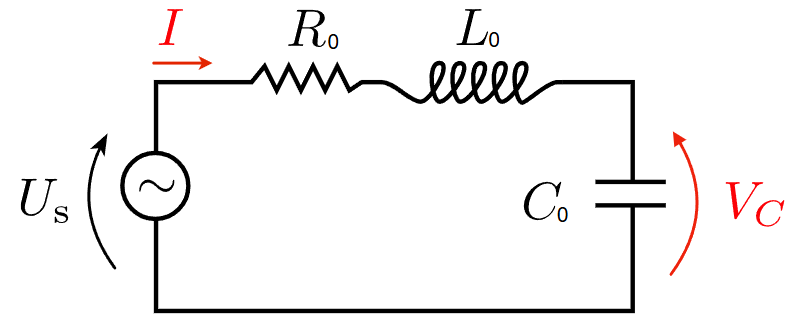
\includegraphics[width=0.8\textwidth]{pic/lab2/RLC.png}
    \caption{Studied RLC circuit}
    \label{fig:RLC_circuit}
\end{figure}

The studied system is the RLC circuit shown in Fig \ref{fig:RLC_circuit}. A set of equations can be derived using Kirchhoff's laws:

\begin{gather}
    u_s(t) = R_0\, i(t) + L_0 \frac{d i(t)}{dt} + \frac{1}{C_0} \int i(t)\,dt\\
    v_C(t) = \frac{1}{C_0} \int i(t)\,dt
\end{gather}

By substituting the second equation into the first one, we obtain:

\begin{equation}
    u_s(t) = R_0\, i(t) + L_0 \frac{d i(t)}{dt} + v_C(t)
\end{equation}

To get to the continuous-time state space representation of this circuit, we need to define the input of the system as $u_s(t)$, its output as $v_C(t)$ and the state vector as:

\begin{equation}
    x(t) = \begin{bmatrix} x_1(t) \\ x_2(t) \end{bmatrix} = \begin{bmatrix} v_C(t) \\ i(t) \end{bmatrix}
\end{equation}

And using:

\begin{equation}
    \begin{cases}
    
    \frac{d V_c(t)}{dt} = \frac{i(t)}{C_0} \\
    \frac{d i(t)}{dt}  =  - \frac{R_0}{L_0} i(t) - \frac{v_C(t)}{L_0}  + \frac{u_s(t)}{L_0}\\

    \end{cases}
\end{equation}

Which finally leads to:


    

\begin{gather}
    \frac{d}{dt} \begin{bmatrix} x_1(t) \\ x_2(t) \end{bmatrix} = \begin{bmatrix} 0 & \frac{1}{C_0} \\ -\frac{1}{L_0} & -\frac{R_0}{L_0} \end{bmatrix} \begin{bmatrix} x_1(t) \\ x_2(t) \end{bmatrix} + \begin{bmatrix} 0 \\ \frac{1}{L_0} \end{bmatrix} u_s(t)\\
    y(t) = \begin{bmatrix} 1 & 0 \end{bmatrix} \begin{bmatrix} x_1(t) \\ x_2(t) \end{bmatrix}
\end{gather}

\begin{equation}
    \Leftrightarrow \hspace{1cm} A_c = \begin{bmatrix} 0 & \frac{1}{C_0} \\ -\frac{1}{L_0} & -\frac{R_0}{L_0} \end{bmatrix}, \hspace{1cm} B_c = \begin{bmatrix} 0 \\ \frac{1}{L_0} \end{bmatrix}, \hspace{1cm} C_c = \begin{bmatrix} 1 & 0 \end{bmatrix}, \hspace{1cm} D_c = 0
\end{equation}

\section{Discrete-time state space model}

To convert this continuous-time state space model to a discrete-time one, we need to select a sampling frequency. As the poles of the system are the eigenvalues of the matrix $A_c$, we can compute them with Matlab, giving:

\begin{equation}
    \begin{cases}
    \lambda_1 \approx (-1 + j 8.1035) x 1e6\\
    \lambda_2 \approx (-1 - j 8.1035) x 1e6
    \end{cases}
\end{equation}

The resonance frequency can be deducted from the eigenvalues computed above.
\begin{align}
    \omega_r &= 8.1035x10^6 \text{rad/s}\\
             &= 1.29 \text{MHz}
\end{align}
The band of interest is therefore chosen to be higher than $1.29$ MHz in order to capture the dynamics of the system. Considering our system being a second-order low pass system, an appropriate sampling frequency would be 10 times higher than $w_r$. Thus $f_s$ is set to $f_s = 12.9$ MHz. The discrete-time state space matrices are computed with Matlab. Two different methods are used: ZOH and tustin.\\
To compare which method is closer to the continuous-time model, the step response of the three models are plotted in Fig \ref{fig:step_response_comparison}.

\begin{figure}[H]
    \centering
    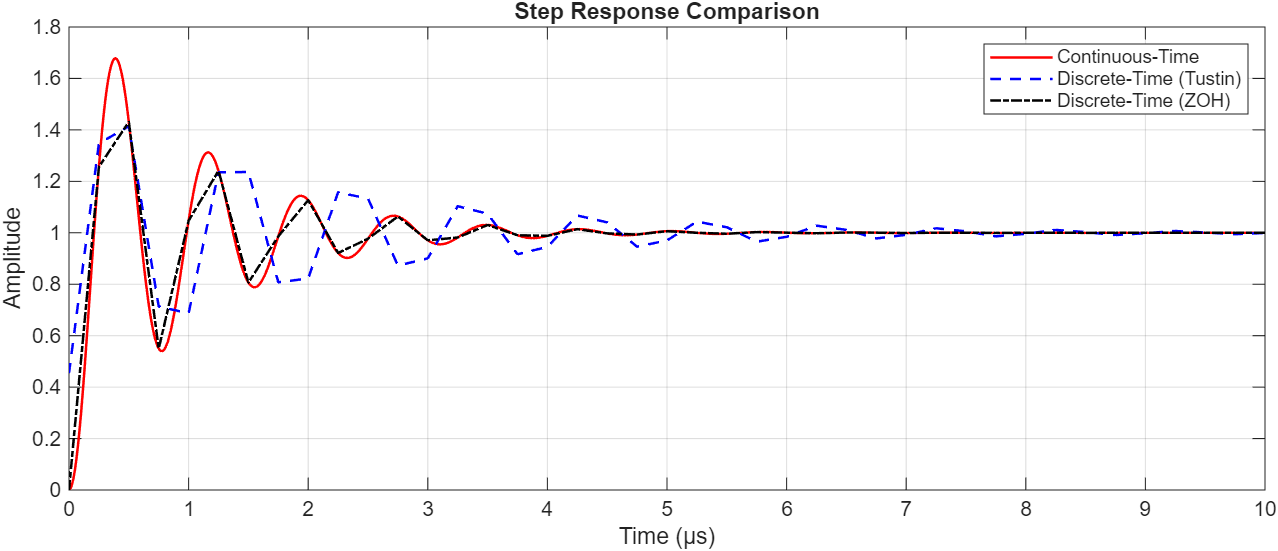
\includegraphics[width=0.8\textwidth]{pic/lab2/stepResponse.png}
    \caption{Step response comparison between continuous-time model and discrete-time models obtained with ZOH and Tustin methods - 4 MHz}
    \label{fig:step_response_comparison}
\end{figure}

\begin{figure}[H]
    \centering
    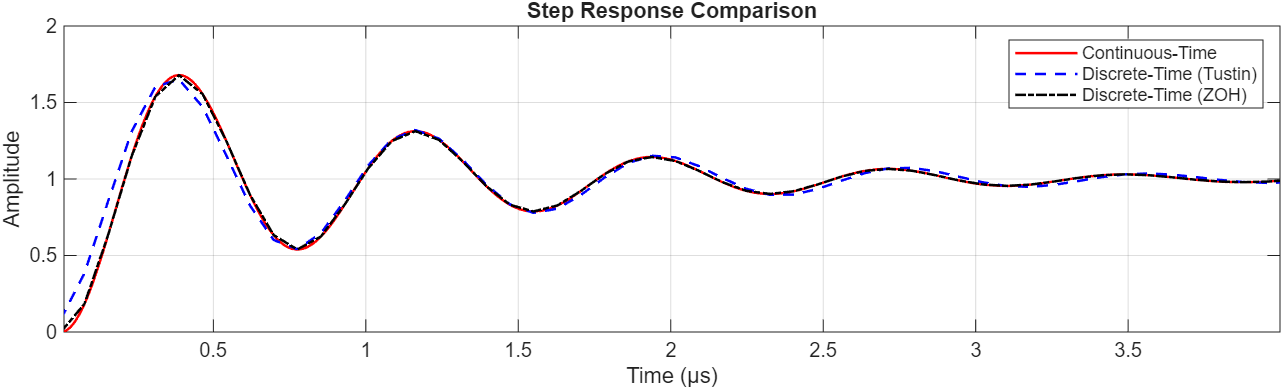
\includegraphics[width=0.8\textwidth]{pic/lab2/stepResponse_am.png}
    \caption{Step response comparison between continuous-time model and discrete-time models obtained with ZOH and Tustin methods - 12.9 MHz}
    \label{fig:step_response_comparison}
\end{figure}

The step response with $f_s = 4$ MHz shows that tustin model presents a mismatch with the continuous-time model (delay introduction in time domain), which is not the case for the ZOH model. The ZOH model is therefore chosen for the following steps. The discrete-time state space matrices are:

\begin{equation}
A_d = \begin{bmatrix}
0.8184 & 22.2414 \\
-0.0133 & 0.6849
\end{bmatrix}, \qquad
B_d = \begin{bmatrix}
0.1816 \\
0.0133
\end{bmatrix}, \qquad
C_d = \begin{bmatrix}
1 & 0
\end{bmatrix}, \qquad
D_d = 0
\end{equation}

The poles of the discrete-time system are also computed by calculating the eigenvalues of the matrix $A_d$ and the system is stable as they are in the unit circle:

\begin{equation}
    \begin{cases}
    p_1 \approx -0.7517 + 0.5407i\\
    p_2 \approx -0.7517 - 0.5407i
    \end{cases}
\end{equation}

To determine whether the system is observable, we can compute the rank of the observability matrix $\mathcal{O}$:

\begin{equation}
    \mathcal{O} = \begin{bmatrix}
    C_d \\
    C_d A_d
    \end{bmatrix} = \begin{bmatrix}
    1 & 0 \\
    0.8184 & 22.2414
    \end{bmatrix}
\end{equation}

Which is of rank 2, meaning that the full space is observable and therefore the states can be fully reconstructed from the output measurement.  Kalman filter can therefore reconstructes both states from the output.

\section{Simulink simulation}

The Simulink model is shown in Fig \ref{fig:simulink_model}. The input is white Gaussian noise with zero mean and variance of 1V. There is also process noise $R_{v_{sim}}$ and measurement noise $R_{n_{sim}}$ which are respectively equal to:

\begin{equation}
    R_{v_{sim}} = \begin{bmatrix}
    0.025 & 0 \\
    0 & 10^{-6}
    \end{bmatrix}, \hspace{1cm} R_{n_{sim}} = 0.0025
\end{equation}

\begin{figure}[H]
    \centering
    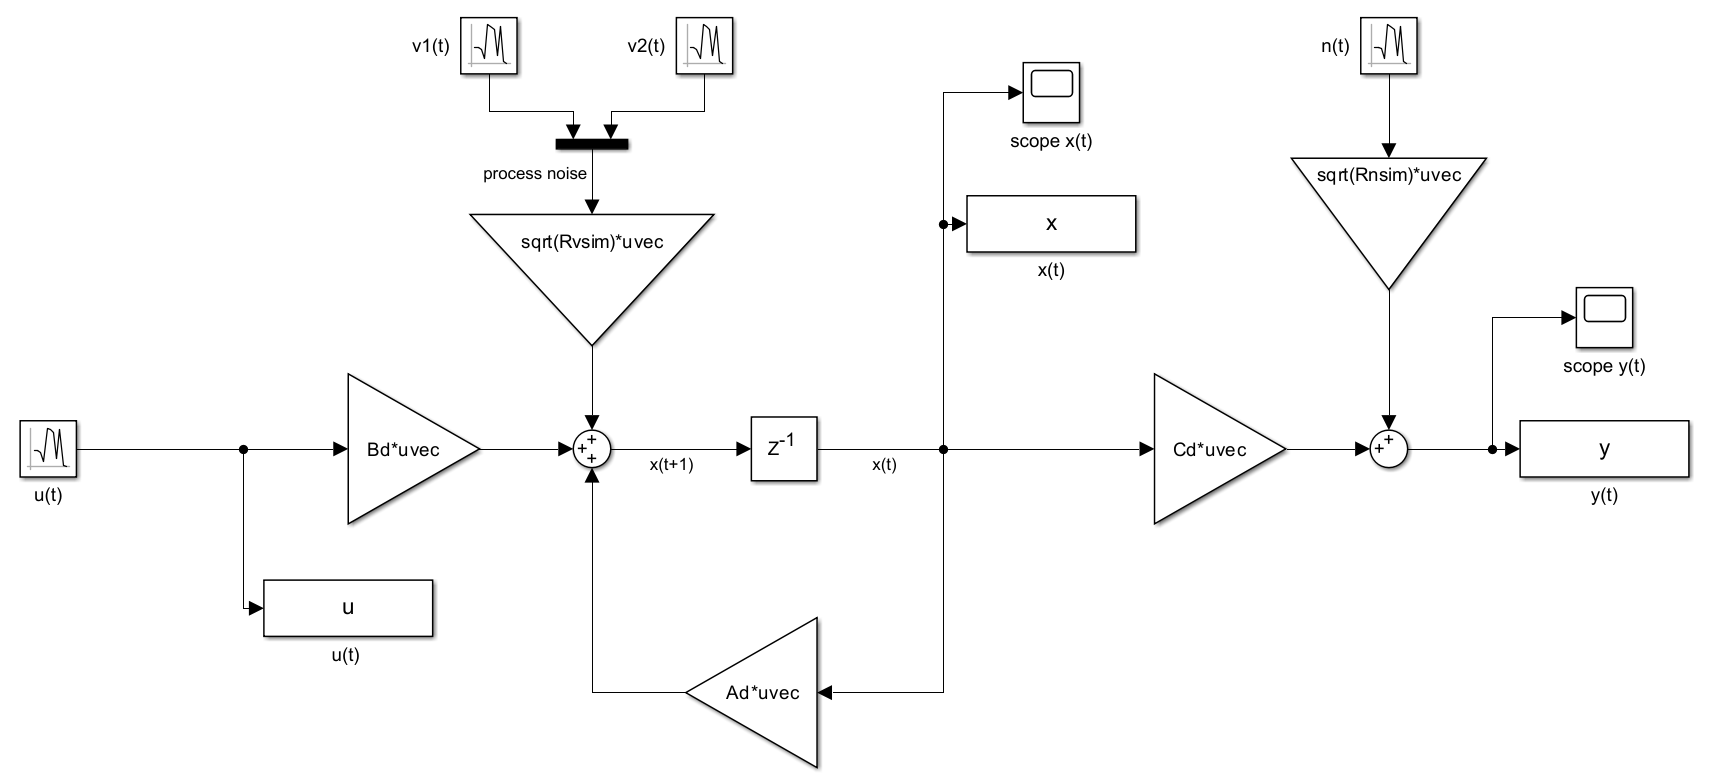
\includegraphics[width=0.9\textwidth]{pic/lab2/simulinkModel.png}
    \caption{Simulink model of the discrete-time state space system}
    \label{fig:simulink_model}
\end{figure}

\section{State estimation}

The state estimation is performed in two ways: a simple prediction based on the model, and a Kalman filter. Both methods are implemented in Matlab as follows:
\begin{lstlisting}[language=Matlab, basicstyle=\ttfamily\footnotesize, keywordstyle=\color{blue}, commentstyle=\color{darkerGreen}, stringstyle=\color{red}]
for itr = 1:size(xin, 1)-1
    % prediction only
    xPred(:, itr+1) = A * xPred(:, itr) + B * uin(itr, :);

    % Kalman
    Q = A * P(:, :, itr) * A' + Rv; % prediction covariance
    K(:, itr+1) = Q * C' / (C * Q * C' + Rn); % Kalman gain
    P(:, :, itr+1) = (eye(size(A, 1)) - K(:, itr+1) * C) * Q; % updated covariance

    prediction = A * xKalman(:, itr) + B * uin(itr, :);
    measurement = (yin(itr+1) - C*prediction - D*uin(itr+1, :));

    xKalman(:, itr+1) = prediction + K(:, itr+1) * measurement;
end
\end{lstlisting}

And those state estimates are compared to the true state, obtained from the Simulink model. The results are shown in Fig \ref{fig:state_estimation}. It can be observed that the error on the state estimation $V_c$ is approximately $25$ dB lower when using the Kalman filter compared to the simple prediction method (open loop observer).
 In the other hand, the differnece between the normalized error for the second state $I$ with Kalman prediction and the open loop observer is much less - around $10$dB.
 The reason will be explained below in the discussion section.

\begin{figure}[H]
    \centering
    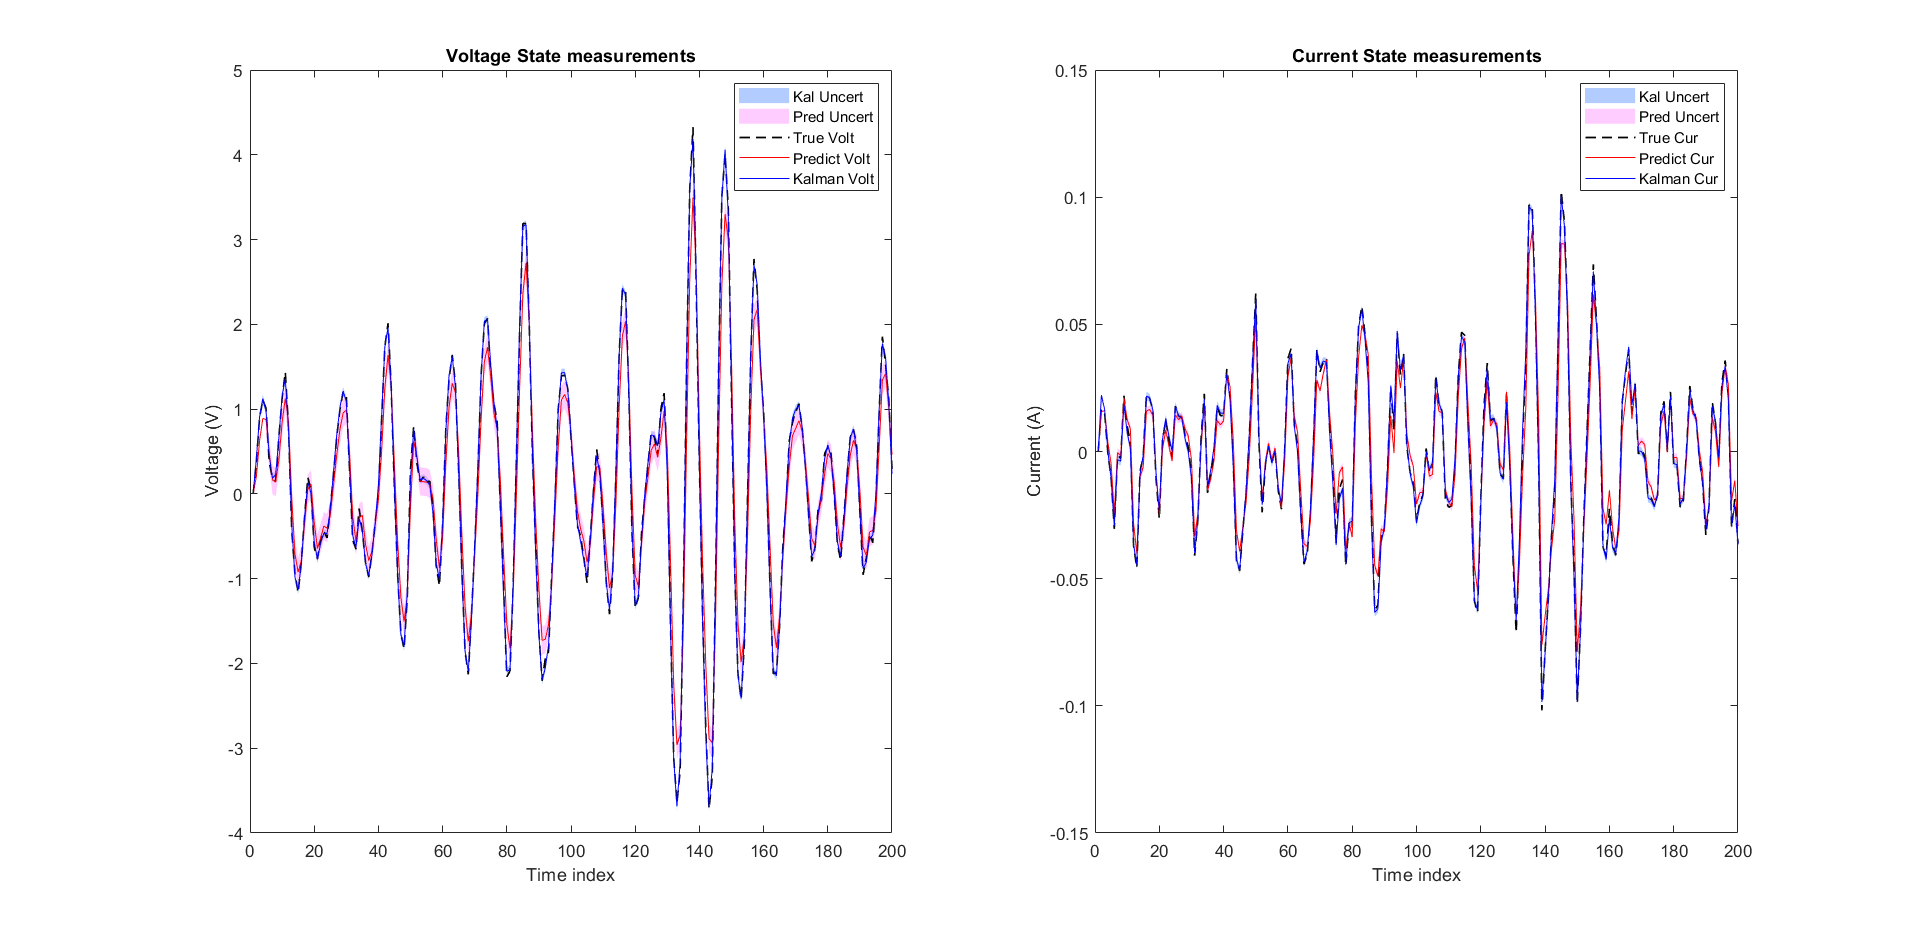
\includegraphics[width=0.9\textwidth]{pic/lab2/kalmanTrueParam_am.png}
    \caption{State estimation comparison between simple prediction and Kalman filter}
    \label{fig:state_estimation}
\end{figure}

\begin{figure}[H]
    \centering
    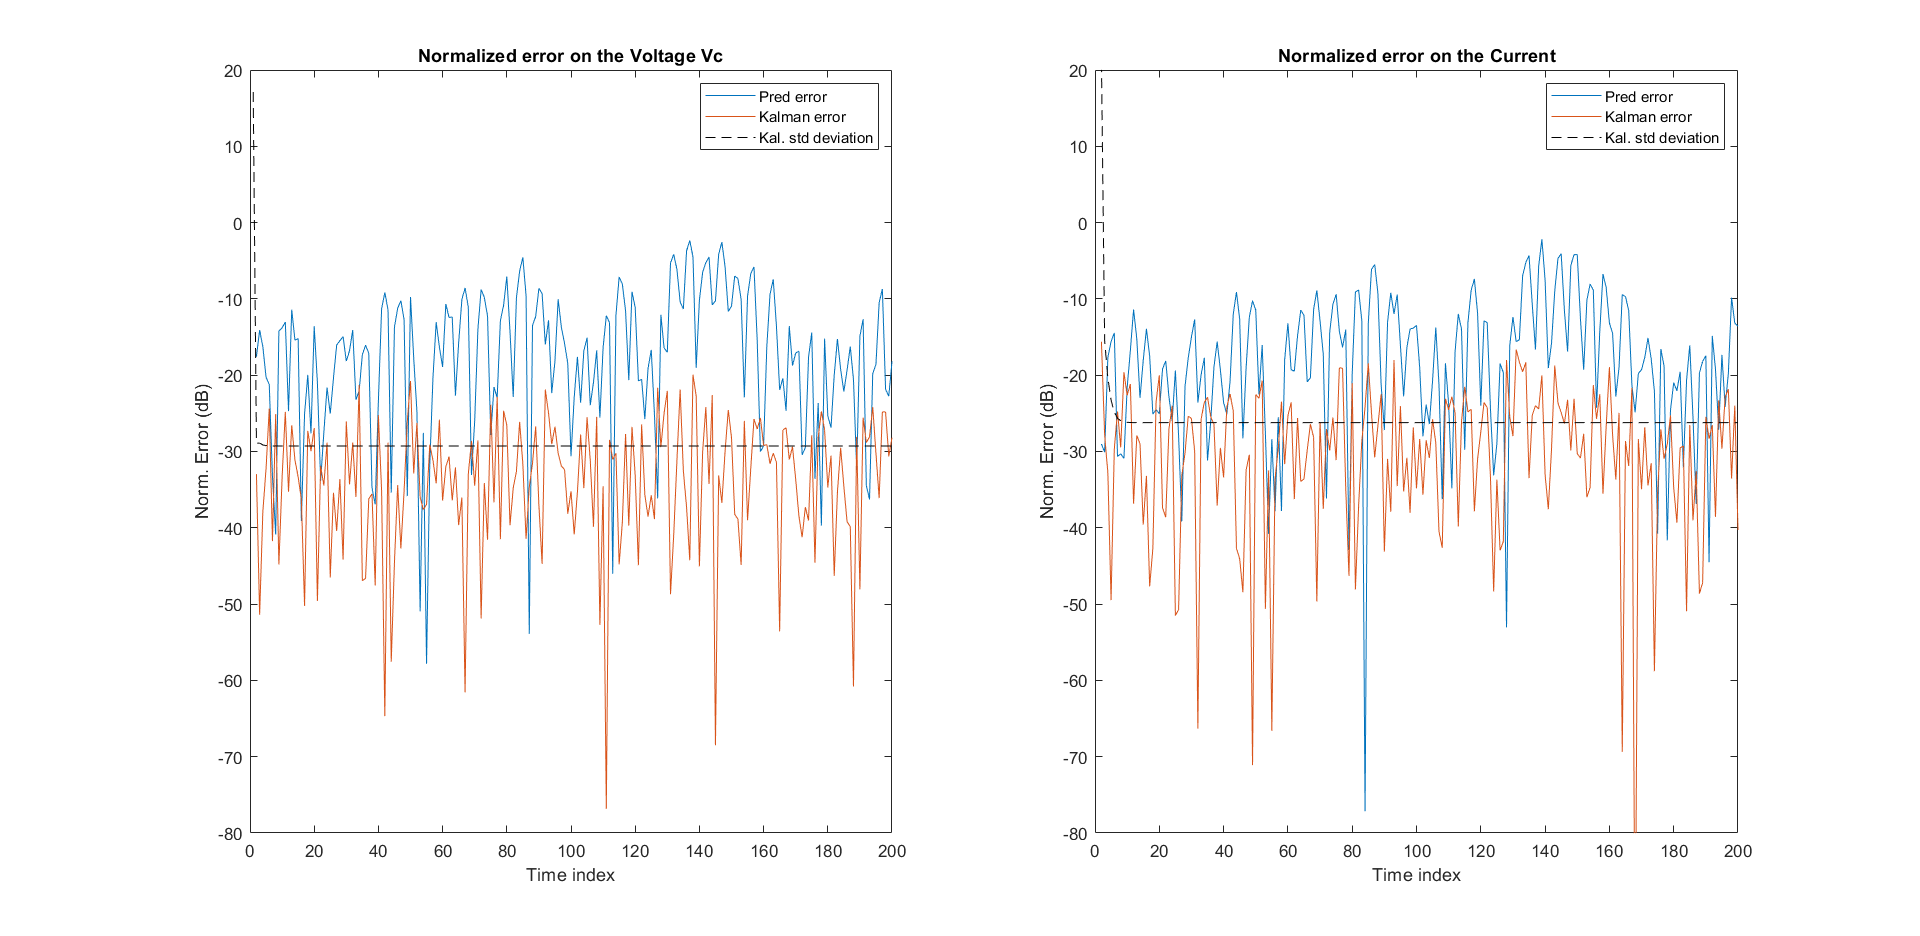
\includegraphics[width=0.9\textwidth]{pic/lab2/kalmanTrueParam_error_am.png}
    \caption{Normalized error comparison between simple prediction and Kalman filter}
    \label{fig:state_estimation}
\end{figure}

To compare the robustness of both methods, the true parameters of the system are modified and the state estimation is performed again. Only the normalized state error plots are shown. \\
On fig \ref{fig:state_estimation_wrong_A} the introduced error on the model ($A = 2 A_{\text{true}}$) makes the model unstable - $|\rm I\!R (\lambda_{obs})| > 0$ . The Kalman filter allows to maintain a stable state thanks to its feedback mechanism (the gain K moves the eigenvalues in the Z-domain and make the observer stable). \\
The impact of a wrong initial condition $x_0$ is shown in Fig \ref{fig:state_estimation_wrong_x0}. Both methods seem to have no significant difference compared to the case with exact initial conditions on fig \ref{fig:state_estimation}. \\
Fig \ref{fig:state_estimation_wrong_Rv} and Fig \ref{fig:state_estimation_wrong_Rn} show the effect of wrong process and measurement noise covariances. In both cases, the estimates are not significantly affected, but the estimated standard deviation is higher than with the true parameters. The standard deviation increase will be also discussed in the conclusion section.

\begin{figure}[H]
    \centering
    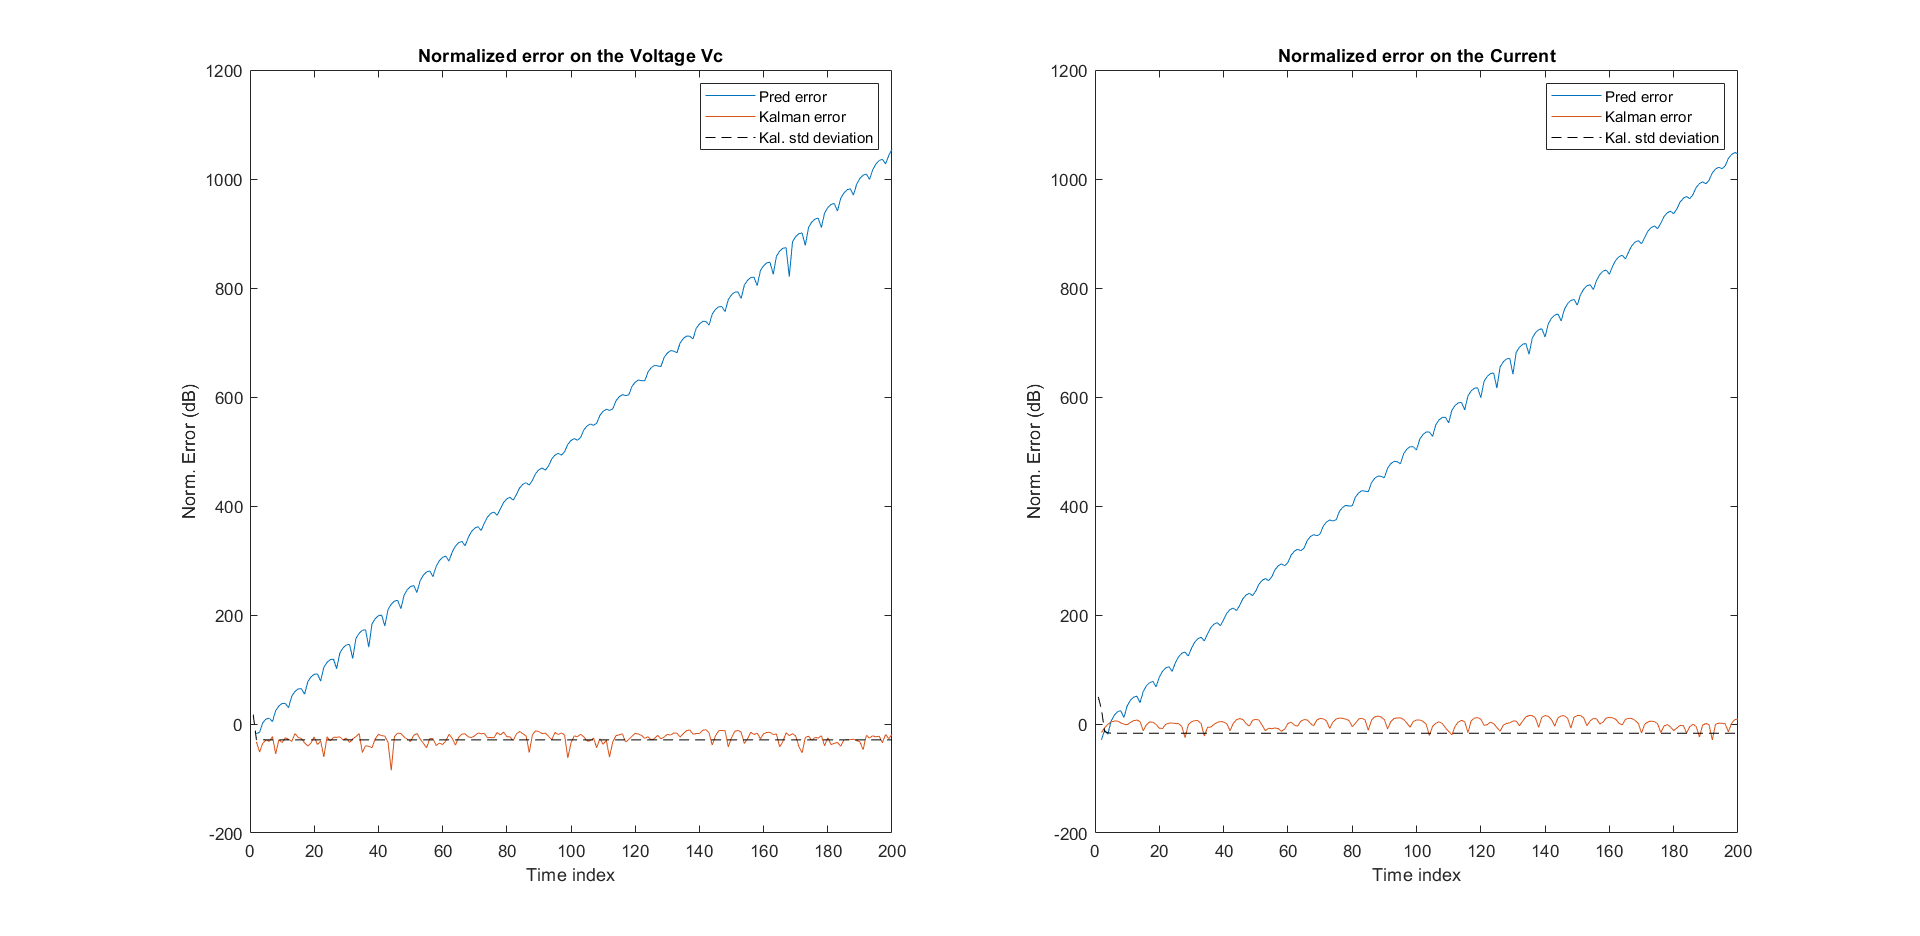
\includegraphics[width=0.9\textwidth]{pic/lab2/kalmanWrongA_am.png}
    \caption{State estimation comparison with $A = 2 A_{\text{true}}$}
    \label{fig:state_estimation_wrong_A}
\end{figure}

\begin{figure}[H]
    \centering
    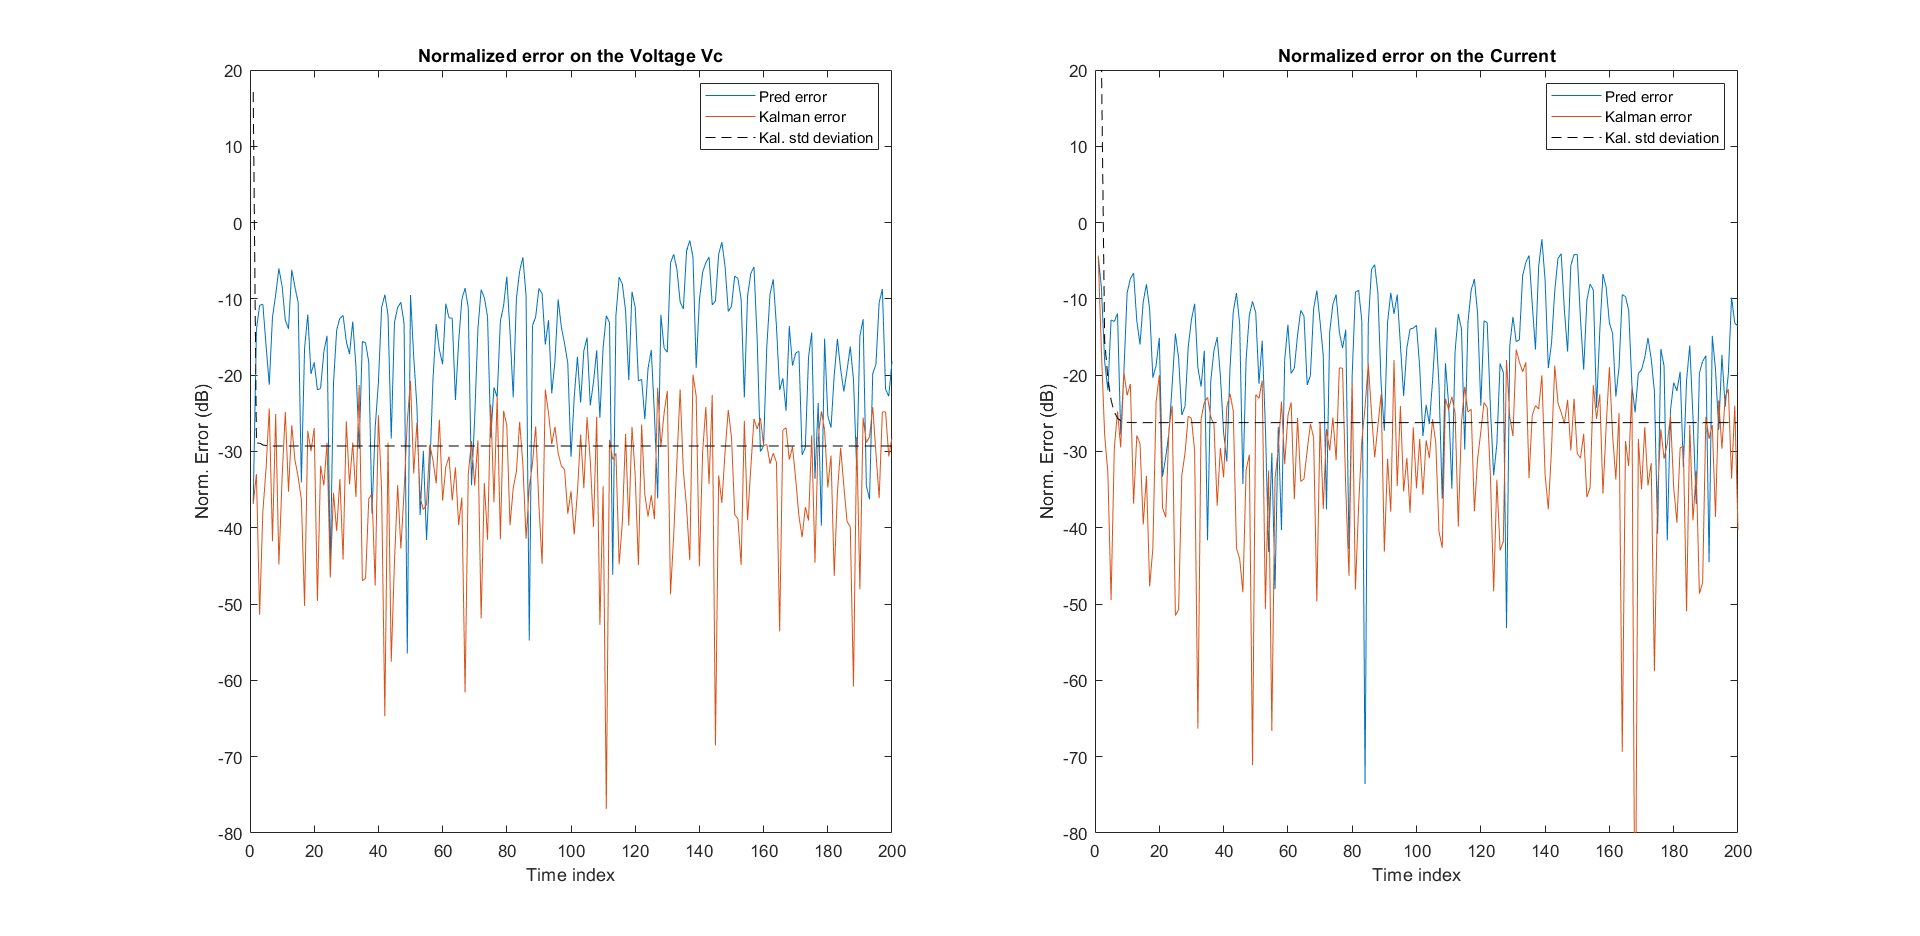
\includegraphics[width=0.9\textwidth]{pic/lab2/kalmanWrongX0_am.png}
    \caption{State estimation comparison with $x_0 = [0.02; 0.02]$ instead of $x_0 = [0; 0]$}
    \label{fig:state_estimation_wrong_x0}
\end{figure}

\begin{figure}[H]
    \centering
    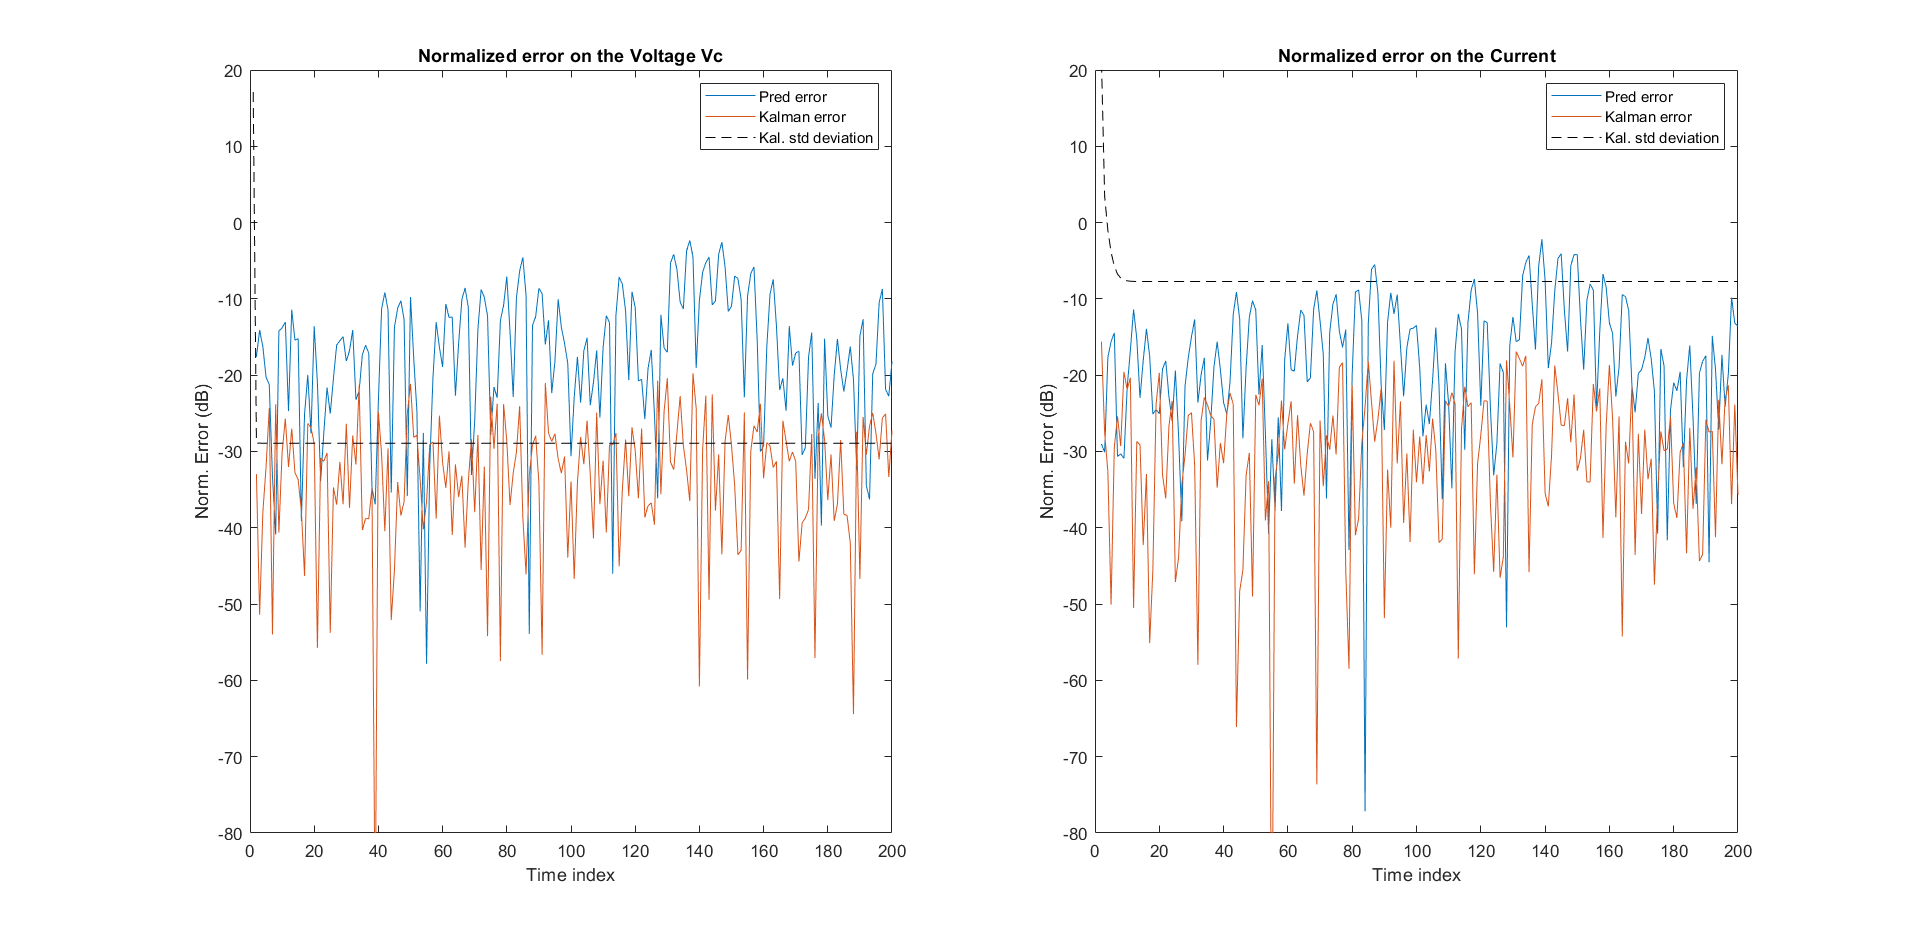
\includegraphics[width=0.9\textwidth]{pic/lab2/kalmanWrongRv_am.png}
    \caption{State estimation comparison with $R_v = 100 R_{v_{\text{true}}}$}
    \label{fig:state_estimation_wrong_Rv}
\end{figure}

\begin{figure}[H]
    \centering
    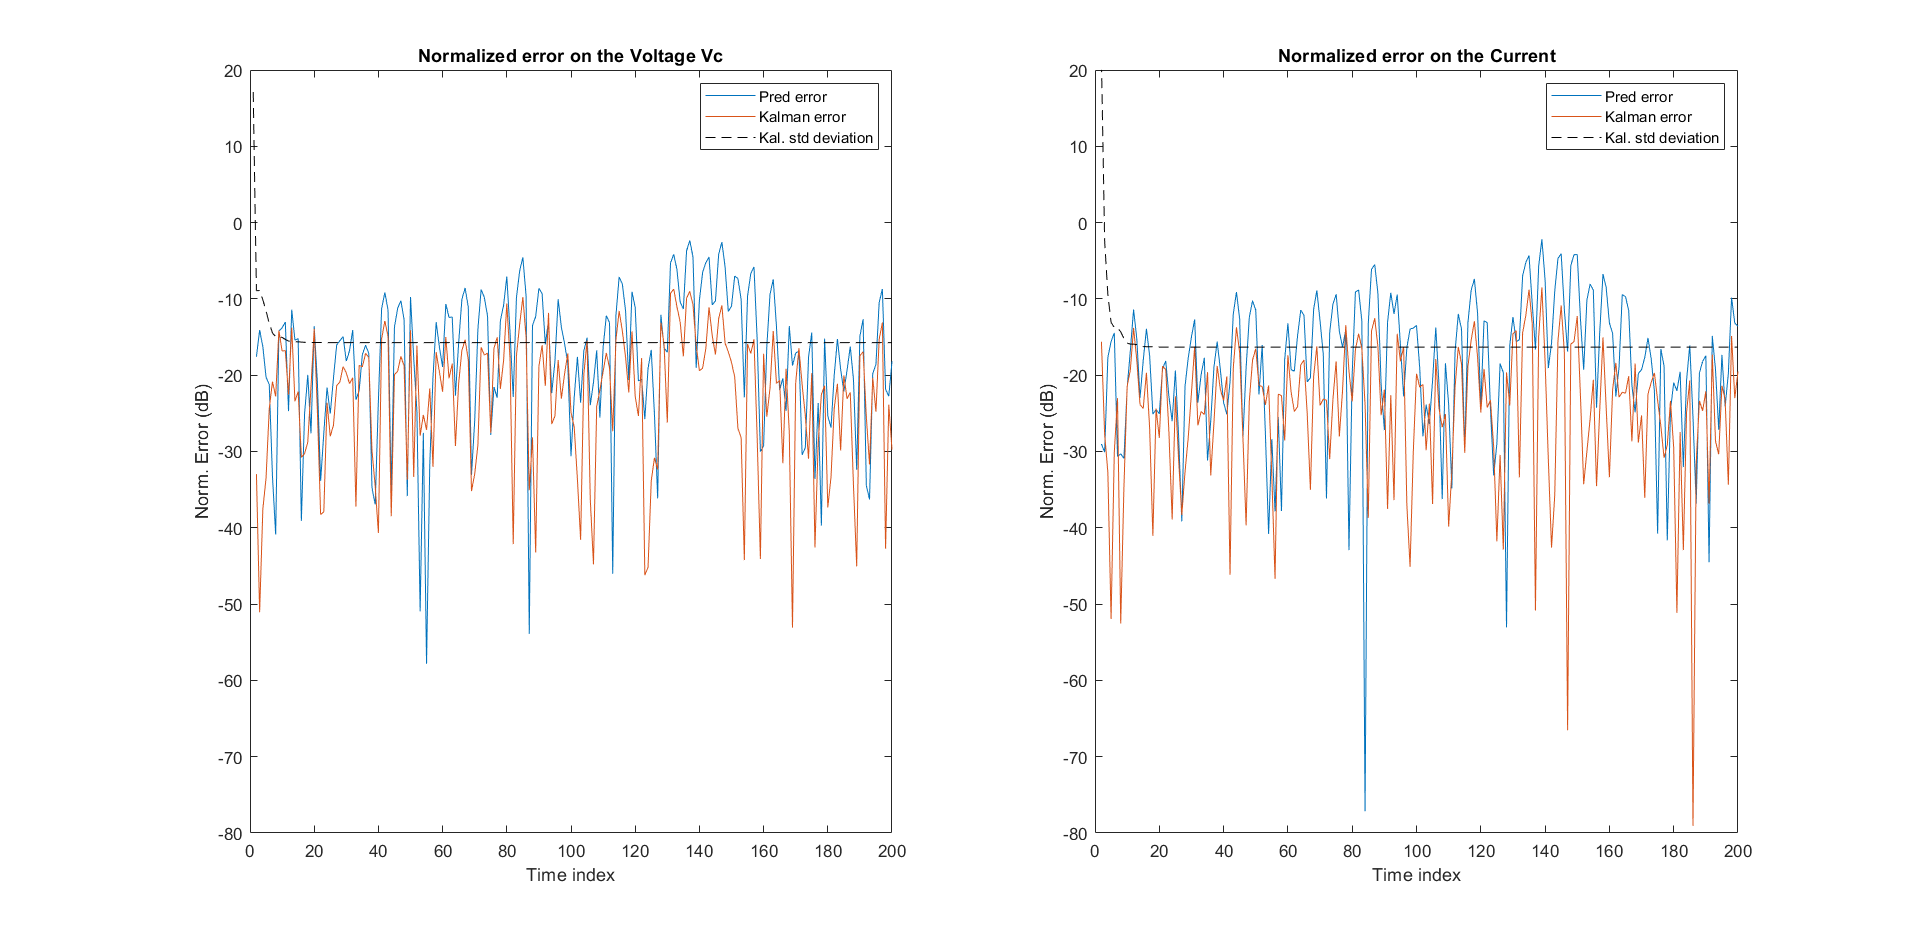
\includegraphics[width=0.9\textwidth]{pic/lab2/kalmanWrongRn_am.png}
    \caption{State estimation comparison with $R_n = 100 R_{n_{\text{true}}}$}
    \label{fig:state_estimation_wrong_Rn}
\end{figure}


\section{Conclusions}

\subsection{Which method performs better?}

Method b (the Kalman filter) performs better. 
In the experiments run from matlab the Kalman filter produces much smaller state estimation error and converges to the true state independant of the initial condition, 
whereas the open‑loop prediction remains biased and has larger steady‑state error. 
(In our test runs the Kalman filter reduced the estimation error by a margin on the order of tens of dB relative to the open‑loop prediction.)


\subsection{Which method is more robust?}

The Kalman filter is more robust in the presence of measurement noise and uncertain initial states: 
it adapts its estimates using incoming measurements and reduces bias that the predictor cannot correct.
However, the Kalman filter is sensitive to model mismatch and to incorrect tuning of the noise covariances: 
large model errors degrade its performance (but typically it still outperforms the naive predictor). 

In short, Kalman = more robust to noise and initial state, but still requires a reasonably accurate model and sensible covariance tuning.

\subsection{Is there a difference in performance between the estimate of the first state (capacitor voltage) and of the second state (current) for method a? And for method b? Why?}

\subsubsection{Method a. Naive prediction - open loop observer}

The capacitor voltage and current exhibit comparable state estimation accuracy, both showing similar normalized error levels.  One might expect the current state estimate to show a higher sensibility to noise than the voltage state estimate ( asthe capacitor voltage is calulated through current integration and would tend to low pass high frequency components as introduced by the noise) .
Nevertheless, the discrete-time state model matrix $A_d$ shows a strong coupling between the states:
\begin{equation}
A_d = \begin{bmatrix}
0.8184 & 22.2414 \\
-0.0133 & 0.6849
\end{bmatrix}
\end{equation}

In particular, the voltage state at t+1 exhibit a high dependence with the previous current state at time t compared to the previous voltage state (the off-diagonal parameter $a_{12} = 22.2414$ is much higher than $a_{11} = 0.8184$ !).
Because of this strong coupling, the error in current state estimation is propagated to the voltage state one step later leading to similar error levels in both estimations.

\subsubsection{Method b. Kalman prediction}

As explained previously, the Kalman predictor behaves as a closed-loop observer.  Unlike the open-loop predictor it continuously corrects its state estimates using the information contained in the output measurement.
Since the discrete-time state output matrix $C_d$ is 

\begin{equation}
C_d = \begin{bmatrix}
1 & 0 
\end{bmatrix}
\end{equation}

Only the capacitor voltage $V_c$ is directly measured at the output.  The current state estimatation is corrected indirectly, in a same pattern as done with the open loop, through the dynamic coupling with the voltage state.
This dynamic coupling exhibiting a weak coupling as shown by the off-diagonal component $a_{21} = -0.0133$ :

\begin{equation}
A_d = \begin{bmatrix}
0.8184 & 22.2414 \\
-0.0133 & 0.6849
\end{bmatrix}
\end{equation}

The error on the current state estimate is therefore reduced compared to the naive prediction but to a lesser extent compared to the voltage state which benefit from the direct measurement feedback.

\subsection{What are the effects of the covariance matrices on the Kalman gain?}

The Kalman gain K depends on the covariance of the predicted state \(Q\), the measurement matrix C and the measurement noise covariance \(R_n\) via following relation
\[
K_{t+1} \;=\; Q_{t+1}\,C^\top\,(C\,Q_{t+1}\,C^\top + R_n)^{-1}.
\]

and where covariance on the estimated state \(P_{t+1}\) and covariance on the predicted state \(Q_{t+1}\) are computed using follwing relationships:
\[
P_{t+1} \;=\; (I - K_{t+1}\,C)\,Q_{t+1} 
\]
\[
Q_{t+1} \;=\; A\,P_t\,A^\top + R_v.
\]

Thus, intuitively:
\begin{itemize}
    \item Increasing the measurement noise \(R_n\) makes the denominator larger and therefore reduces \(K\): the filter trusts the model more and the noisy measurements less.
    \item Increasing the covariance on the predicted state \(Q\) tends to increase \(K\): larger uncertainty in the state estimate makes the filter rely more on measurements.
    \item Increasing the process noise covariance \(R_v\) increases \(Q\) and hence increases \(K\).
    \item Initial \(P\) affects the transient gains.
\end{itemize}
Edge cases: as \(R_n\to 0\) the gain tends to the (pseudo‑)inverse, while as \(R_n\to\infty\) the gain tends to zero and the filter behaves like a simple predictor.

\subsection{Advantages, limitations and suggestions for practical situations in which you would use the Kalman filter ?}

The feedback mechanism of the Kalman filter offers multiple advantages.
\paragraph{Accuracy improvement, stabilization and automation}
As seen previously, the Kalman prediction owns the benefit of the closed loop observer which allow to place the eigenvalues in the unitary circle thanks to its closed-loop correction mechanism.\\
This feedback modifies the dynamics of the observer through the Kalman gain $K$, effectively shifting the observer poles through:

\begin{equation}
A_{obs} = A-KC
\end{equation}

With K computed based on the estimated uncertainty level encoded in the state covariance matrix $P$.

It is a significant advantage compared to open loop observer which stability depends directly on the poles of the matrix $A_d$ (leading to unstability in the case of $A_d = 2 x A_d$) but also to other closed loop observers like the Luenberger observers where the poles placement
are moved manually by the designer's / user's choice - $(A+LC)$.

Those properties make the Kalman observer automatically stable with moderate noise but also highly flexible to noise variation.

\paragraph{Robustness to the initial state errors and noise}

The previous simulations shows also a robustness to incorrect initial state conditions.  Choosing a suffisiantly large initial covariance P at the time instant $t0$ impose a high uncertainty on the initial state to the observer. Kalman observer will therefore emphasize the measurement output to estimate the state at the time instant $t+1$.\\
The modulation of the gain $K$ through the covariance matrix $P$ (and indirectly $Q$) secures a quick convergence to the true value even with wrong $x_0$.\\
In addition, the observer will adjust the gain $K$ in function of the process noise covariance and the measurement noise covariance giving an optimal balance between the model and the measurement information. Nevertheless, this specific link between $R_v$ and $R_n$ may lead to some 
limitations..

\paragraph{Limitations}

Although it is a powerful tool to track the state, Kalman filter has also limitations :

\begin{itemize}
    \item We just discussed about how robust is the Kalman observer to the noise but this property is true if we assume that $R_v$ and $R_n$ reflect the reality.  If the noise covariances matrices are purely tuned, the observer will return biased estimates or may become unstable.
          Also the $R_n = 100 x R_n$ simulation highlights how excessive noises levels drag the observer to behave like an open-loo^p observer.
    \item The second limitation is inherent to any observers.  The observation requires \underline{observability}.  It means that states are only recoverable if they are observable from the output $y$. Additionally, an observer relies on the correctness of the state space representation ($A_d, B_d, C_d, D_d$).
          Kalman predictor cannot compensate for complete unfaithful representation to the system reality even if it shows robustness for limited mismatch ($A_d = 2 x A_d$ experiment).
\end{itemize}

\subsubsection{Practical situations}

Today, Kalman predictor is used in many situations.  We discussed during the course about Artemis program and the rocket trajectory correction but Kalman is also used today for much simpler experiments :
\begin{itemize}
    \item Automating watering fields with limited number of moisture sensors.
    \item Robotic control system (Hidden state estimation).
    \item Autonomous driving (localization).
    \item Finance (Inflation rates calculation through measured income data by example)
    \item etc.
\end{itemize}